\subsection{Автокодировщик для обнаружения аномалий}

Также для решения задачи обнаружения аномалий было рассмотрено применение автокодировщиков (или автоэнкодеров, англ. autoencoder). Представляет собой архитектурный класс искусственных нейронных сетей, которая использует метод обучения без учителя с применением алгоритма обратного распространения ошибки.

В применении автокодировщиков для обнаружения аномалий используется их основное свойство --- необходимость фиксировать в скрытом латентном слое, полученном с помощью кодера (англ. encoder), наиболее важной информации о входном сигнале для его последующего восстановления декодером (англ. decoder). Благодаря этому свойству автокодировщик способен восстанавливать знакомый ему сигнал, считающийся нормальным, и не может восстановить аномальный сигнал, содержащий неизвестные паттерны. Это свойство и заложено в основе применения автокодировщиков для обнаружения аномалий.

Рассмотрим нейронную сеть автокодировщика с единственным скрытым слоем. Она будет иметь кодер и декодер, заданные соотношениями (\ref{h_def}) и (\ref{z_def}), соответственно.

\begin{equation}\label{h_def}
    \overline{h} = \sigma(W_{xh} \overline{x} + \overline{b_{xh}}),
\end{equation}

\begin{equation}\label{z_def}
    \overline{z} = \sigma(W_{hx}\overline{h} + \overline{b_{hx}}),
\end{equation}
где $W$ и $\overline{b}$ --- вес и смещение (англ. bias) нейронной сети, \\
$\sigma$ --- функция нелинейного преобразования.

Кодер в уравнении (\ref{h_def}) отображает входной вектор $\overline{x}$ в скрытое представление $\overline{h}$ с помощью нелинейного преобразования. Декодер в (\ref{z_def}) отображает скрытое представление $\overline{h}$ обратно в $\overline{z}$ исходного пространство с помощью того же преобразования, что и кодер. Разница между исходным входным и восстановленным векторами называется ошибкой восстановления, как показано в формуле (\ref{e_def}).

\begin{equation}\label{e_def}
    e =  \lVert \overline{x} - \overline{z} \rVert.
\end{equation}

Автокодировщик обучатся минимизировать $e$. Алгоритм обучения нативного автоэнкодера показан в алгоритме~\ref{alg:AE_train}, где $f_{\phi}$ и $g_{\theta}$ - многослойные нейронные сети для автокодировщика.

\begin{algorithm}[htp!]
    \caption{Стандартное обучение автокодировщика} \label{alg:AE_train}
    \SetAlgoLined %% Это соединяет линиями логические части
    \KwData{Набор данных $\overline{x_1}, ..., \overline{x_n},\ n < k$}
    \KwResult{ обученные $f_{\phi}$ и $g_{\theta}$ }
    
    Инициализировать параметры $\phi$ и $\theta$ \\
    \While{ не достигнута сходимость $\phi$ и $\theta$}{
        // Вычисление суммарной ошибки восстановления. \\
        $E = \sum\limits_{i = 1}^n\lVert \overline{x_i} - g_{\theta}(f_{\phi}(\overline{x_i})) \rVert$ \\
        $\phi,\ \theta \leftarrow$ Обновление параметров с помощью градиента $E$ (например, стохастический градиентный спуск) \\
    }
    \Return{$f_{\phi}$, $g_{\theta}$}
\end{algorithm}

Обнаружение аномалий на основе автокодировщика --- это метод обнаружения аномалий на основе отклонений, использующий обучение с частичным привлечением учителя (англ. semi-supervised learning). Он использует ошибку восстановления в качестве оценки аномалии. Точки данных с высокой значением $e$ считаются аномалиями. 

Для обучения автоэнкодера используются только данные с нормальными экземплярами. После обучения автоэнкодер будет очень хорошо восстанавливать нормальные данные, но не сможет сделать этого с аномальными данными, с которыми автоэнкодер не сталкивался. Алгоритм \ref{alg:AE_detector} демонстрирует обнаружение аномалий с использованием ошибок восстановления автокодировщиков.

\newpage

\begin{algorithm}[htp!]
    \caption{Обнаружение аномалий на основе автокодировщика} \label{alg:AE_detector}
    \SetAlgoLined %% Это соединяет линиями логические части
    \KwData{ \\
        Набор \textbf{нормальных} данных $X' \subset X,\ |X'| = n < k$, \\
        Набор неразмеченных данных (потенциально аномальных)  $\overline{x'_1}, ..., \overline{x'_l} $, \\
        Метки классов $Y = \{y_1,\ y_2\}$, где $y_1$ --- <<аномальный>>, \\
        $\phantom \qquad\qquad\qquad\qquad\qquad\qquad\qquad\quad\ y_2$ --- <<нормальный>>, \\
        Порог ошибки $\epsilon$.
    }
    \KwResult{ значение ошибки восстановления $e =  \lVert \overline{x} - \overline{z} \rVert$ }
    
    $\phi,\ \theta \leftarrow$ обучить, используя набор <<нормальных>> данных $X'$ \\
    \For {$i := \overline{1,\ l}$} {
        $error(i) = \lVert \overline{x_i} - g_{\theta}(f_{\phi}(\overline{x_i})) \rVert$ \\
        \eIf{$error(i) > \epsilon$}{
		$\overline{x_i}$ помечается, как принадлежащий классу $y_1$
	}{ 
		$\overline{x_i}$ помечается, как принадлежащий классу $y_2$
	}
    }
\end{algorithm}

Рассмотрим архитектуру нейронной сети автокодировщика, представленной на рисунке \ref{fig:autoencoder-scheme}, которая может быть применена для обнаружения аномалий сетевого трафика.

\begin{figure}
  \centering
  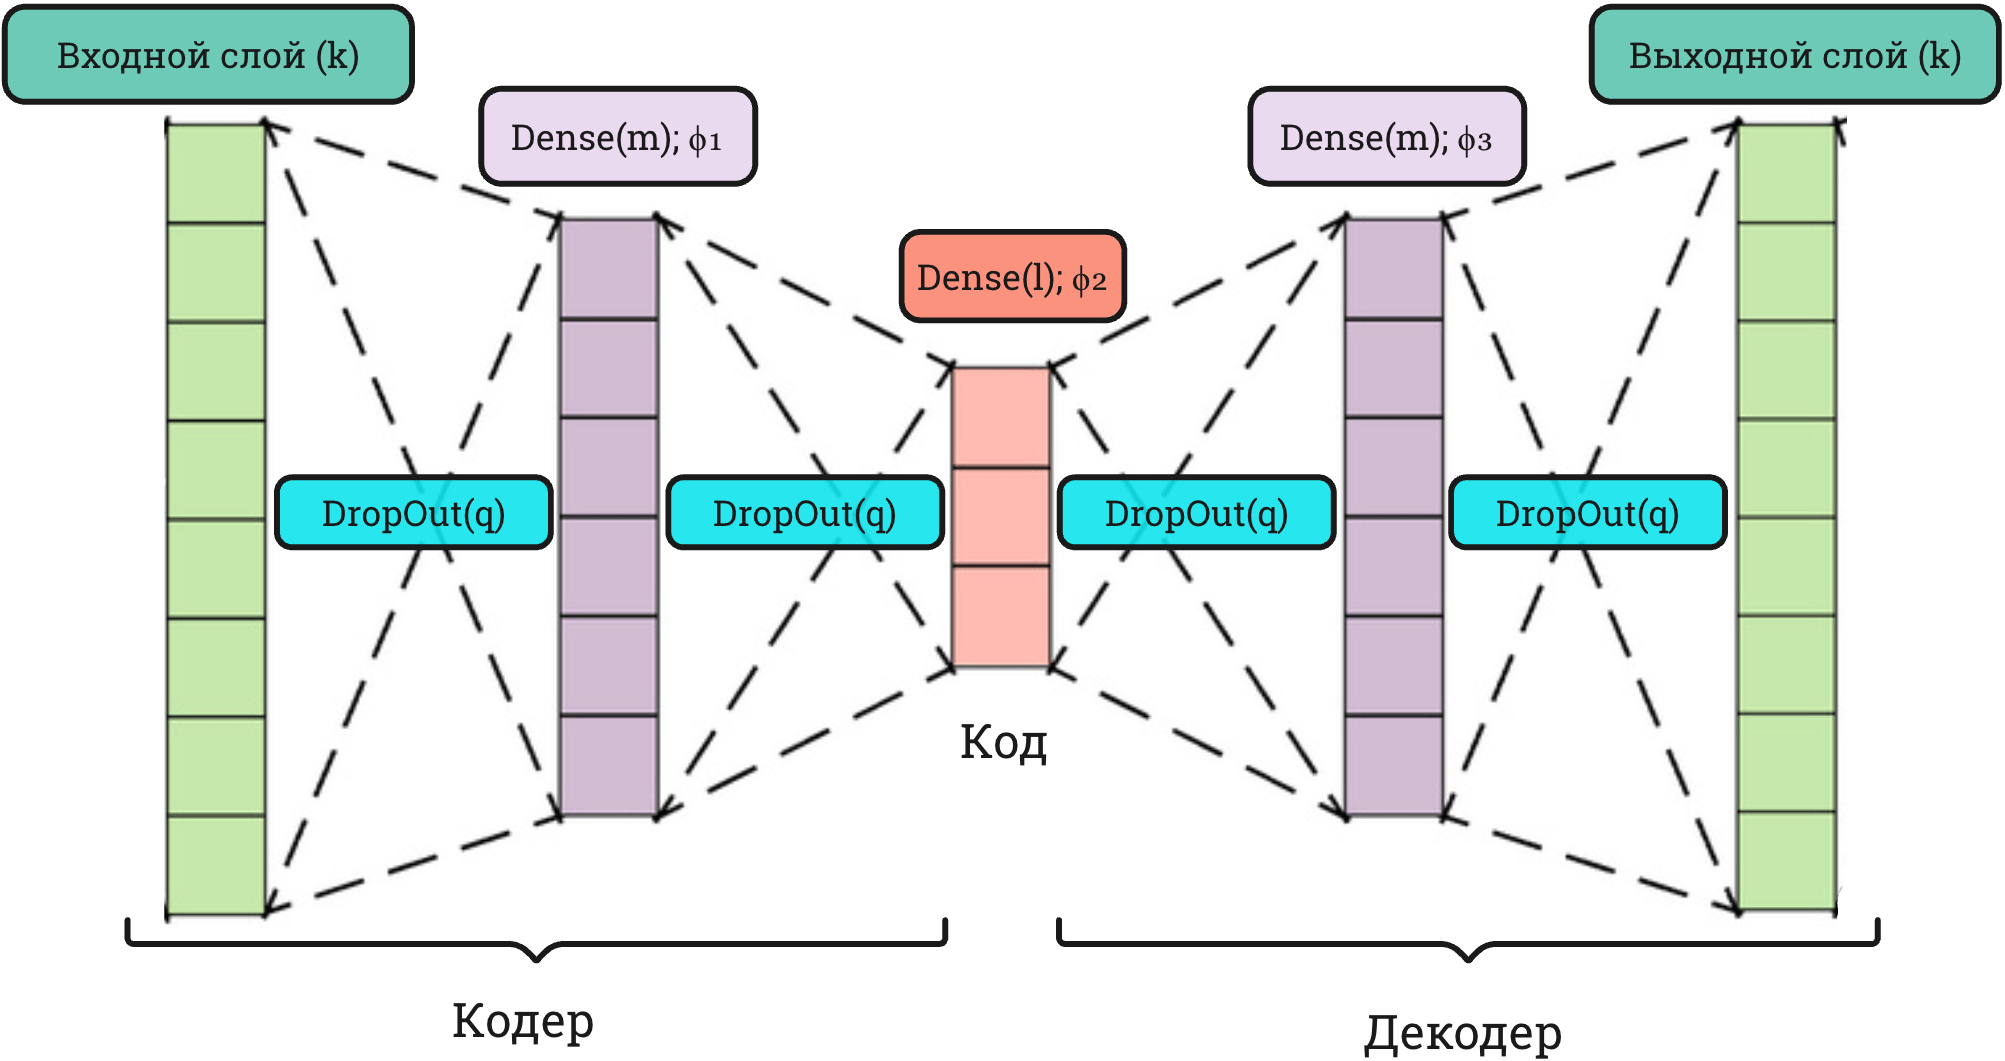
\includegraphics[scale=0.23]{inc/images/autoencoder-scheme.png}
  \caption{Архитектура искусственной нейронной сети автокодировщика для обнаружения аномалий в сетевом трафике}
  \label{fig:autoencoder-scheme}
\end{figure}

Входной и выходной слои имеют количество нейронов по числу признаков, извлечённых в элементы $X$ из множества $T$ по формуле (\ref{X_def}). Скрытые слои энкодера и декодера содержат $m$ и $l$ нейронов соответственно.

Каждый слой использует функции активации $\phi_1$, $\phi_2$ и $\phi_3$ для введения нелинейности в модель. Примером хорошо зарекомендовавшей себя функции активации может послужить линейный выпрямитель (или полулинейный элемент, англ. \textit{Rectified linear unit}, ReLU), представленный формулой (\ref{relu_def}). Она монотонна, что гарантированно делает выпуклой поверхность ошибок, ассоциированную с одноуровневой моделью. Также ReLU --- гладкая, то есть имеет монотонную производную, что в некоторых случаях обеспечивает более высокую степень общности.

\begin{equation}\label{relu_def}
    \phi(x) = 
    \begin{cases}
        0, &\ \text{если } x < 0, \\
        x, &\ \text{если } x \ge 0. \\ 
    \end{cases}
\end{equation}

Также в автокодировщике применяется метод регуляризации \textit{Dropout} с параметром $q \in (0;\ 1)$, что помогает предотвратить переобучение, случайным образом отключая $q \cdot 100\%$ нейронов во время обучения. 

Обучение автокодировщика может осуществляться с использованием функции потерь $MSE$ (англ. \textit{Mean Squared Error} --- среднеквадратичная ошибка), которая измеряет разницу между входными данными и восстановленными данными. Далее результаты восстановления декодера сравниваются с входным слоем для оценки аномальности экземпляра данных. Среднеквадратичная ошибка определяется соотношением $MSE = \sigma^2$, где $\sigma$ --- стандартное отклонение, ранее определённое в формуле (\ref{standard_deviation}).
